\subsection{Content Filtering}
The implementation of content filtering constitutes of Python scripts which handle all of the data preprocessing, training of the model and predicting of the post categories. As with abuse detection, this makes use of multiple Python libraries including Sci-kit learn \cite{scikit:home}, NLTK \cite{nltk}, Numpy \cite{Numpy} and Pandas \cite{Pandas}, which provide machine learning models and objects for processing datasets. The code is divided between three files, each of which handle a stage of the machine learning process: preprocess.py, train.py and predict.py.

\subsubsection{Data Preprocessing}
The file preprocess.py cleans the textual post so that it can be used in either the training or predicting processes. The implementation of the cleaning is shown in figure \ref{fig:content-clean}. The function carries out a list of commands sequentially, each of which remove aspects of the post which are unwanted. The package \textit{p}, whose \texttt{clean()} function is used is the tweet-preprocessor package \cite{TweetPreprocessor}. This function removes any Twitter entities, except for the hashtags, from the post, including mentions, URLs and emoticons. Since Fidelis is using the same tagging system as Twitter, the same cleaning function can be applied to Fidelis posts. The $WordLemmatizer$ object is from the NLTK library, which processes lemmatizes each of the words in the post to reduce the noise created as a result of different forms of the same word. 

\begin{figure}[H]
\centering
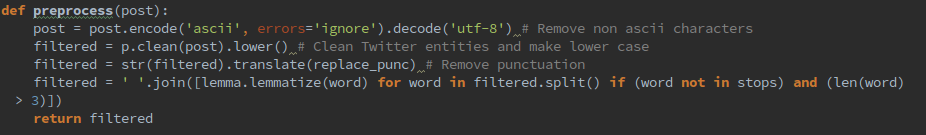
\includegraphics[width=\textwidth]{Images/Implementation/content-clean}
\caption{Function that cleans a post}
\label{fig:content-clean}
\end{figure}

The only part of the design algorithm \ref{alg:content-filter-cleaning} which is not performed by this function is the check that the length of the preprocessed string is less than 20. This is instead performed by both the training and prediction functions. Figure \ref{fig:content-preprocess} shows the preprocessing which occurs in the training file.

\begin{figure}[H]
\centering
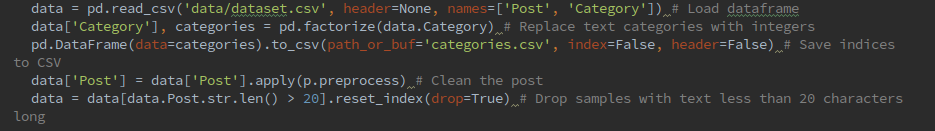
\includegraphics[width=\textwidth]{Images/Implementation/content-preprocess}
\caption{Preprocessing of content before training}
\label{fig:content-preprocess}
\end{figure}

In addition, the extraction of features from the post is performed in the training and prediction files, because they are performed on the dataset as a whole rather than on each individual post. The count vectorization and tf-idf transformations are parsed into the pipeline shown in \ref{fig:imp-content-train}, using the Sci-kit learn objects $CountVectorizer$ and $TfidfTransformer$. The $CountVectorizer$ also creates the uni- and bi-grams which are present in the dataset.

\subsubsection{Model Building}
Figure \ref{fig:imp-content-train} shows how the Stochastic Gradient Descent model is trained, including the pipeline which extracts features from the dataset. Whereas the pipeline stage creates the model, the $fit()$ function is what initiates the training of the model on the training data.

\begin{figure}[H]
\centering
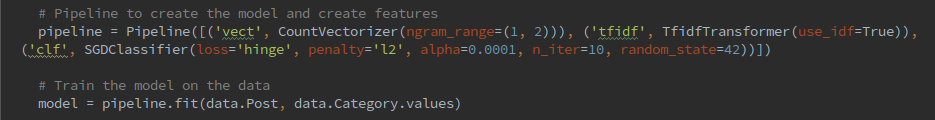
\includegraphics[width=\textwidth]{Images/Implementation/content-train}
\caption{Training the model}
\label{fig:imp-content-train}
\end{figure}

However, as well as building the model using the entire dataset, cross-validation is also implemented, where the model is only trained on 90\% of the data at a time. Figure \ref{fig:content-cv} shows how the cross-validation is performed. This is performed alongside the training of the model in train.py. The function \texttt{cv\_val\_score()} is imported from Sci-kit learn, and handles the splitting of the dataset and the training/testing of each cross-validation model to calculate the score.

\begin{figure}[H]
\centering
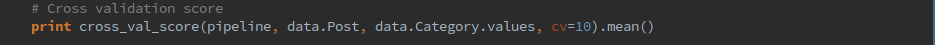
\includegraphics[width=\textwidth]{Images/Implementation/content-cv}
\caption{Cross-validating the model}
\label{fig:content-cv}
\end{figure}

\subsubsection{Predicting Topics}
The prediction algorithm \ref{alg:content-filter-predict} can be divided into two sections: predicting the initial topic of the post and updating the topic as a result of user input. To predict the initial topic, a request to the API is made to predict the category of the post. Using the \texttt{exec()} PHP function, the predict script is run, which returns the topic of the post. The PostController PHP file which handles the API call then adds the tag-category pairs to the category\_tag table.

The user is then able to amend the chosen topic of their posts. A bootstrap modal is opened when the user wishes to change the topic and another request to the API is made when the change is made, which updates the tag categories in the database.